% global change “ – ’
 
\chapter{Interbranch quarrel in comparative perspective}
\label{ch:sopInPerspective}
\chaptermark{Comparative interbranch quarrel}

%abstract
%This chapter provides a birds-eye view on how I study the legislative process in systems of separation of power (sop).  Two decision-making principles coexist in sop: one requiring the powers to concur on new policy, another establishing exceptions to concurrent consent.  There is a tendency in the literature to overlook exceptions (unilateralism), biasing appraisals of sop systems.  The chapter also incorporates these principles into an abstract framework---the amplified game of sop---which represents the essential rules of policy-making.  The components of this game are isolated to get a sense of the substantive claims that can be produced with each.  The chapter also introduces a discussion on the motivation that guides politicians in choosing their actions.  Motivation will be the clue to begin constructing a unified model of the legislative process in systems of sop. 

There is a classic distinction in comparative politics between two forms of democratic government, the parliamentary and the presidential.  The primary attribute of parliamentarism is that the legislative and executive powers of government are fused; under presidentialism there is a separation of these powers \citep{lijphart.1984}. There has been much controversy over the pros and cons of fusion and separation of power.  

Debate has taken place mostly at the theoretical level, with claims remaining, for the most part, unaccompanied by convincing empirical evidence.  But even on the theoretical front the state of the discussion is inconclusive, due in great part to the difficulty of isolating the independent effect that broad governmental forms have on government performance from those of a myriad of smaller institutional details.  Asking whether fusion is better or worse than separation of power may be too broad a question.  

My research branches out of this intellectual tradition.  I shall not, however, engage in a discussion of pros and cons.  In this thesis I focus, instead, on \emph{how the legislative process operates in systems of separation of power in the Americas}.  Policy is, for the most part, written as a set of pieces of legislation.  The legislative process is consequently the primary arena where governmental actors make decisions affecting the citizenry.  

In this chapter I present an outline of my argument.  The chapter is divided into 9 short sections that are organized in the following fashion.  

\emph{Separation of Power}.  Section 1 situates decision-making in a presidential or ``separation of power'' system in the context of the establishment of checks and balances in government, highlighting the dilemmas this raises for constitutional designers.  A definition of separation of power will be found in this section.  Section 2 introduces two principles of decision-making that, I argue, characterize any system of separation of power.  The principles are concurrent consent and unilateralism.  Section 3 offers a quick critical assessment of the relevant literature; I argue that there is a tendency, especially acute in the comparative literature, to omit the institutions of unilateralism in their conception of the legislative process.  

The Legislative Process.  Next, I concentrate on sketching the conceptual tools for the study of the legislative process in a generic separation of power polity.  Section 4 introduces a general or macro framework---the amplified game of separation of power---knitting together the theoretical parts of my thesis (as well as theoretical extensions that I will develop in the near future).  I then break the big framework into three smaller, analytically tractable, subsidiary models, all of which branch off from the encompassing frame (they are sub-games).  Sections 5, 6, and 7 provide outlines of the subsidiary models: the setter sub-game; the conditional decree sub-game; and the vetoes in the shadow of decrees sub-game.  These sketches introduce the basic building blocks with which my succeeding arguments are constructed, and in each of these three sections I also discuss the interesting substantive claims that are made based on this sort of model, foreshadowing what I will do in subsequent chapters or future extensions of the work.  

Actors' motivation.  Section 8 begins by synthesizing the stylized structures in which politicians interact in my model.  I then introduce a discussion on motivation: what is it that moves politicians who play these stylized games of the legislative process?  This brief discussion will anticipate the contents of the final chapter of the thesis, an attempt to synthesize two literatures on the legislative process (one in Anglo-American politics, another in comparative politics) that do not communicate despite dealing with essentially the same issues.  

Section 9 concludes by summarizing my approach to the study of the legislative process into a research design, presenting the questions that guide the thesis, defining the dependent and main independent variables, establishing a null hypothesis, and offering a general description of the methodology.\footnote{As will be evident, I have written this introduction in such a way that it addresses the contents of a large research agenda.  Some parts of the argument are not developed in chapters to follow; I do indicate, nonetheless, which pieces of argument are developed in subsequent chapters and which are projects.}

\section{What is separation of power?}
\label{s:whatSOP}

In framing a government which is to be administered by men over men, 
the great difficulty lies in this: you must first enable the government to 
control the governed; and in the next place oblige it to control itself
—Madison (1788, Federalist 51). \nocite{madison.1788}

Political theorists for at least two and a half centuries have been seeking institutional devices to constrain the capacity of government to violate the rights of the citizenry.  Three eminent figures in this school of thought, \citet{locke.1690}, \citet{montesquieu.1748}, and \citet{madison.1788}, favored the separation of policy-making power as an effective way to curb the all-too-human inclination of rulers to exploit the ruled --- ``il faut que le pouvoir arr\^ete le pouvoir'' suggested the second (163), which the third translated almost literally as ``ambition must be made to counteract ambition'' (322).  Yet these thinkers were also the first to recognize what their detractors have subsequently been emphasizing \citep[eg.][]{bagehot.1867,wilson.1884,romero.1893}: if separation of power results in an increase in the representativeness of policy it also implies an inevitable loss in the government's decisiveness---perhaps, in the spirit of Madison, the central dilemma in democratic theory.  

Constitution-writers in the independent nations of the American continent, by following the example set forth by the U.S.\ at the end of the 18th century, seem to have valued increased representativeness more than they feared the possibility of governmental indecisiveness.  In drafting the institutions of government they chose to include checks and balances in some or all of four common modalities: (1) separation of legislative and executive powers; (2) separation of legislative power between two chambers representing different constituencies; (3) breaking policy into national and sub-national jurisdictions; and (4) separation of the enactment from the interpretation of law \citep[see][]{cox.mccubbins.2001,tsebelis.1995}. 

In this thesis I will be studying separation of power in the first modality only: the disjunction between the ability to write policy and the ability to turn it into law.  Constraining attention in this manner results in a narrow definition of separation of power throughout the thesis: \emph{by separation of power I will always mean separation of the legislative branch from the executive branch of government}.  In this sense, I am following the classic distinction I introduced at the opening of the chapter.  

By this definition, a separation of power system becomes synonymous with a presidential system.  I prefer the term ``separation of power'' (which I will often abbreviate as sop) because ``presidential'' is a term open to ambiguous meanings.\footnote{Thus for example, it is not uncommon for the literature to refer to a system with an abnormally strong or imperialist president as an excessively ``presidential'' one, or ``hyperpresidential''.  The literature, for example, refers to the centrality of Mexico's president as presidencialismo \citep{carpizo.1978,weldon.1997}. Yet by hyperpresidential, it could also be understood that the system in question boldly separates the authorities of the branches in a way that actually renders the president rather weak.  Sop avoids this confusion; I thank Matthew Shugart for pointing this out to me.}  In reviewing the literature, however, I retain the common term to make it easier to recognize original arguments.  

\section{Two decision-making principles in separation of power}
\sectionmark{Two decision-making principles}

The rules of separation of power are a mixture of two principles of decision-making that, in their pure form, are antithetical.  The principles in question are concurrent consent and unilateralism.  The principle of concurrent consent prescribes that new policy requires the approval of the two branches of government: any change in policy sought by the executive branch can be rejected or ``vetoed'' by the legislative branch; symmetrically, the executive can veto any proposal by the legislative.  The principle of unilateralism, on the other hand, allows one branch to overcome a rejection by the other: unilateral powers effectively entitle each branch to establish new policy by itself (under certain circumstances).  

In their pure form, it is easy to see that unilateralism and concurrent consent are mutually exclusive maxims.  Yet constitutional engineers over the last centuries have devised hybrid forms of these principles which can actually coexist.  This hybridization results in a mixture that may well be called concurrent consent with restricted unilateralism.  Below I argue that much of the debate on separation of power has failed to recognize the presence of elements of unilateralism in the structure of decision-making.  

Concurrent consent is incorporated into a sop constitution by empowering the legislative and the executive with an authority to veto new policy.  This gives rise to the executive veto and the congressional veto, faculties giving each branch the power to enforce the status quo ante before any new decision becomes law.  This mutual veto power is the feature of sop constitutions that is recognized by all scholarly literature, both of Anglo-American and comparative politics.  

Restricted unilateralism, on the other hand, is less often acknowledged as part of separation of power.  Restricted unilateralism is incorporated into a sop constitution in two main modalities, overrides and decrees.  

The override authority is the legislative branch's means of setting aside an executive veto in order to clear the way for new policy.  An override mechanism becomes a restricted form of unilateralism by requiring the legislative assembly to reveal extraordinary strength before it is effective: if normal passage of policy requires a plurality of votes, overriding an executive veto typically requires a larger degree of consensus, some super-majority.  The larger the super-majority required, the more restricted becomes this form of unilateralism.  

The decree authority is the executive branch's means of circumventing a congressional veto.  Executive decrees permit the president to set new policy without the need of a statute written by the legislative assembly \citep[9]{carey.shugart.1998}.  A decree is a restricted form of unilateralism because, after some time, the legislative branch may decide the fate of any executive decree.  The easier it is for the assembly to rescind or amend a decree, the more restricted becomes this form of unilateralism.  

\begin{table}
\begin{center}
\begin{tabular}{c|c|c}
\emph{Authority}        & \emph{Executive}             &  \emph{Legislative}              \\
\emph{by which$\ldots$} & \emph{branch}                &  \emph{branch}                   \\ \hline
$\ldots$ branch rejects & \textbf{executive veto}      & \textbf{legislative veto}        \\
a proposal              & Ch.\ 3 veto in US states     &  Ch.\ 9 reacting to executive    \\
by the other            & Ch.\ 5 stunts Chile/Mex.     &  decrees in Argentina            \\ \hline
$\ldots$ branch over-   & \textbf{unilateralism}       & \textbf{veto override}           \\
comes a rejection       & Ch.\ 6 urgency in Chile      &  Ch.\ 4 hopeless vetoes          \\
by the other            & Ch.\ 7 exec.\ coalition      &  Ch.\ 8 overrides in Brazil      \\
\end{tabular}
\caption{Veto power and unilateral provisions, side to side}\label{t:twoPrinciples}
\end{center}
\end{table}

Table \ref{t:twoPrinciples} summarizes how the two hybrid principles of decision-making are combined into the concept of separation of power that I use throughout this research.  Note that in this framework executive decrees are to legislative vetoes what veto overrides are to executive vetoes.  Both are concrete mechanisms by means of which concurrent consent and unilateralism are allocated, more or less symmetrically, to the branches of a separation-of-power government. 

Different separation of power systems can be thought of as mixtures of different proportions of concurrent consent and restricted unilateralism among the branches.  A sweeping literature documents the numerous dimensions over which the formal institutions of sop vary from one constitution to another \citep{shugart.carey.1992,mainwaring.shugart.1997,carey.shugart.1998}. So, for example, unilateralism is quite limited and lopsided towards the legislative branch in certain systems.  This is the case, for example, in the U.S., Mexico, and Costa Rica, where the executive has no formal decree authority to overcome a congressional veto, and where overrides of executive vetoes become effective only after two-thirds of each house of the assembly has voted favorably.  Other systems of sop have less limited and more symmetric unilateral provisions.  Examples of this are Brazil (since 1988) and Colombia (since 1991), where the executive is explicitly granted a decree-making authority and the legislative assembly is entitled to override vetoes more easily, by absolute majority only.  Still other systems tilt the balance of unilateral power towards the executive branch.  Such is the case in Argentina (since 1994), where the executive holds a decree power while the assembly's override power requires a two-thirds vote \citep[150--5]{shugart.carey.1992}.

\section{Unilateralism overlooked: the pressure boiler and the safety valves}
\sectionmark{The pressure boiler and safety valves}

As I mentioned above, there is a remarkable tendency in the literature to ignore the presence of the restricted unilateralism principle in separation of power.  This tendency is milder and easier to account for in some works than in others.  The Anglo-American literature falls on the mild end: it does take one form of unilateralism into consideration but disregards the other.  Models of inter-branch relations in the U.S. typically feature the veto-override faculty of the assembly \citep{lee.1975,rohde.simon.1985}; they omit executive decree authority \citep[exceptions are][]{sala.1998,moe.howell.1999}.  Given that the U.S. constitution grants no formal decree authority to its executive, and that Anglo-American politics research focuses solely on the case of the U.S., it becomes easy to elucidate the omission of this form of unilateralism---it's simply not needed to account for the case of the U.S.  

The tendency to neglect restricted unilateralism is starkest in the Perils of Presidentialism literature in the field of comparative politics.  This literature, largely derived from recent work by Juan Linz, has hypothesized the highly destabilizing potential of any presidential constitution.  Presidential systems, it is argued, by electing the branches of government separately and for fixed terms, promote discord between them; at the same time they fail to provide constitutional mechanisms to resolve such disputes \citep{linz.1990,linz.valenzuela.1994}.  Unilateralism, in both its forms, is discarded as part of the Linzian conception of SoP, and this has been inherited by the voluminous research that the framework inspired \citep{linz.valenzuela.1994}.  

The probable explanation behind this neglect of unilateral provisions is the search for parsimony.  Linz chose to explicitly ignore the smaller institutional details of SoP, as can be inferred from the following quote:

\begin{quote}
Without going into the \emph{complexities} of the relationship between the executive and the legislature in different presidential regimes, the relative dangers of predominance of one or the other, and the capacity to veto or stalemate decisions on legislation, there can be no doubt that presidential regimes are based on a dual democratic legitimacy and that no democratic principle can decide who represents the will of the people in principle \citep[][7, emphasis added]{linz.1994}.
\end{quote}

But, unlike the literature in the Anglo-American Politics field, the omission is puzzling in a comparative perspective.  In fact, the principal claim of those who first took issue with the Linzian argument is that we cannot really understand whether or not this double legitimacy is problematic, and to what extent, without paying attention to the ``complexities'' of separation of power \citep{shugart.carey.1992}.  The rebuttal to the Linzian literature has, in turn, motivated a voluminous research agenda \citep{mainwaring.shugart.1997}.  

A good analogy for the system of policy-making portrayed in the Linzian story seems to be a pressure boiler with no safety valve.\footnote{This evocative analogy was suggested to me by Gary Cox.}  Opposition between the executive and the legislative turns on the gas in the system, putting it under increasing pressure.  Pressure keeps accumulating as long as the branches maintain a disagreement about legislation.  In the absence of constitutional safety valves---i.e. mechanisms to shut off or depressurize the system in case the barometer approaches the red zone---the only way to bring pressure back to normal is by reaching an agreement between the branches---turning off the heat.  If recalcitrance between the branches prevails and no such agreement is reached, the whole system eventually blows up in a democratic meltdown.\footnote{Linz's terms are, actually, pretty suggestive of this pressure boiler with missing safety valves: \begin{quote}who, on the basis of democratic principles, is better legitimated to speak in the name of the people: the president, or the congressional majority that opposes his policies?  [C]onflict is always latent and sometimes likely to erupt dramatically; there is no democratic principle to resolve it$\ldots$  It is therefore no accident that in some of those situations the military intervenes as ``poder moderador'' \citeyearpar[][7]{linz.1994}.\end{quote} On the contrary, when executive-legislative pressure becomes sizeable in a parliamentary system, a government crisis reunifies policy purpose between the executive and the legislature, ‘depressurizing' the system.  This constitutional safety valve avoids the breakdown of democracy.}

The truth is, however, that the institutions of restricted unilateralism in fact equip sop systems with different sorts of devices to avoid explosions.  Legislative overrides, executive decrees, and other ``complexities'' that the Linzian story overlooked need to be brought back in: they constitute the very safety valves of the sop pressure boiler.\footnote{\citet{domingo.morgenstern.nd} list at least a dozen of other formal and informal ``road-clearing devices'', such as congressional monopoly on constitutional amendment (as in Colombia); budgetary bills subject to no executive veto (as in Mexico); agenda-setting tools like the urgency provision in the hands of the executive (as in Chile); etc.}  In the following sections I introduce an alternative framework that takes the safety valves of presidentialism into consideration; this represents one important deviation from the Linzian structure.  

\section{The legislative process as a game of strategy}

How are decisions made under separation of power?  How do the institutions translating the principles of concurrent consent and unilateralism, described in previous sections, interplay?  In particular, how do the congressional and the executive veto powers, the veto-override provision, and executive decree authority determine policy outcomes?  What patterns can we expect from arrangements combining these institutions differently among the branches of government?  Answering these and related questions brings us straight into the realm of the legislative process.  The legislative process includes a wide range of actions leading to and including the enactment of statutes, passage of resolutions, issuing of decree-laws, nominations and confirmations, and so forth.  

I construe the legislative process as a game of strategy played by politicians.  I will call this stylized framework the amplified game of separation of power (or the amplified sop game for short).  Representing decision-making with the tools of game theory is standard procedure in analyses of U.S. politics \citep[eg.][]{shepsle.1979,ingberman.yao.1991,krehbiel.1996,cox.1999,mccarty.2000,cameron.2000}.  It is a much less common research strategy in comparative studies, though it is gaining popularity \citep[eg.][]{huber.1996a,cox.1997,diermeier.feddersen.1998,baron.ferejohn.1989,londregan.2000a}.  I choose the game theoretic approach to the structure and process of policy because it is a particularly useful one.  It forces the analyst to think systematically about who makes collective choices, what actions are available to ``players'' at different stages of the ``game'', and which actions should be chosen in light of pre-defined goals.  Such representation, when used creatively, generates some non-evident and even counter-intuitive conclusions from a set of explicit primitives.  Moreover, deductive reasoning---inherited to game theory by its mathematical formalization---facilitates appraisal of the consequences of altering a model's premises, while assuring that the argument remains logically sound.  

amplified sop is a game for three players.  It begins with a pre-established policy, the status quo (denoted by SQ), which players ``P'', ``L'', and ``V'' jointly decide whether or not to change under rules that I portray in Game Tree \ref{f:amplifiedGame}. Player P represents the president; player L represents a unitary-actor legislature; and player V is the veto-override pivot (whose identity I clarify below).  

\begin{figure}
 \begin{center}
%  \includegraphics[width=\textwidth]{../veto/graphs/amplifiedGameOld.pdf}
  \includegraphics[width=\textwidth]{amplifiedGameOld.pdf}
 \caption{The big tree of separation of power: the amplified sop game}\label{f:amplifiedGame}
 \end{center}
\end{figure}

Player P starts the amplified sop game by choosing one of three available actions: P can propose a bill to the assembly; P can establish new policy by decree; or P can choose to do nothing.  The first choice represents an attempt by the president to make policy by statute (a change from the existing policy SQ to a new one denoted xP).\footnote{For clarification, no assumption is being made so far about the kind of bill proposed by player P; this will be the subject of subsequent chapters.  The subindex P in xP should only be interpreted as referring to the author of the policy proposal, in this case player P.  In the same fashion xL refers to a policy proposal by player L.}  The second choice represents an attempt by the president to establish the new policy xP unilaterally.  The third option represents a president who chooses to retain the status quo.  

Amplified sop ramifies into distinct sub-games depending on the action chosen by P in his or her first move.  I do not describe the sequence of action.  Instead I break exposition into some of the sub-games of amplified sop, devoting the following sections of the chapter to an outline of each (sub-games that I isolate from Game Tree \ref{f:amplifiedGame} have a square in their starting node.)  Before doing so, however, a couple of comments are in order.  

Note first that the model involves an extremely simplified representation of the assembly.  I make collective choice in the amplified sop game analogous to choice by an individual, ignoring lessons against such a practice from the social choice literature \citep{plott.1967,mckelvey.1976,schofield.1983,riker.1980}. There are several ways of circumventing this problem.  One is to make feasible policies fall along a single dimension and then appeal to the median voter theorem to predict collective choice \citep{black.1958,tsebelis.money.1997}.  Another is to appeal to the presence exogenous restrictions that limit the social choice mechanism in a way that brings a stable and predictable equilibrium, such as transaction costs \citep{sloss.1973,lupia.mccubbins.1997} or the division of labor \citep{shepsle.1979}.  A plausible restriction to rely on is political parties as binding constraints that bring enough discipline among their members to render behavior by the collective body predictable \citep{cox.mccubbins.1994}. The elaboration of sub-games in chapters to follow involves unidimensionality; within this assumption, I leave it open for the reader to choose whether player L represents the leader of the party or coalition controlling a majority of seats \citep{cox.mccubbins.2005}, or the median member of a unicameral legislative assembly \citep{krehbiel.1998}.\footnote{If there is an advantage in having the majority in government then there exist good reasons to behave like a party.  There is evidence that majority status is valuable even in a system such as the U.S., where there is a consensus that parties are less meaningful than average.  Democrats lost between \$36,000 and \$60,000 per member in contributions from business PACs only upon losing grip of the House majority in 1994 \citep{cox.magar.1999,cox.magar.nd}.}

Second, let me tell what I will not be doing with this framework.  The principal object of a stylization of the legislative process such as the amplified sop game is to put the analyst in a position to generate interesting logical predictions.  This operation involves finding a game's equilibria, something analogous to ``solving'' the game.  An equilibrium in the game is a set of mutual best-reply strategies (one for every player); stated differently, in equilibrium each player is responding optimally to what the others are doing.  Equilibria are obtained by logical deduction: they follow from a set of premises describing the game's rules, a definition of what motivates every player in the game, and other elements of a more technical nature.  

So far I have provided some of the elements to obtain equilibrium strategies for the game.  I do not intend to solve the amplified sop game in this thesis.  The abundance of ramifications in Game Tree \ref{f:amplifiedGame} yields countless possible combinations of moves, making their analysis a most burdensome task that I leave for the future; I have more modest goals at present.  Despite this, there are at least two good reasons why presenting the amplified sop game has been a useful exercise.  

One is that the richness of amplified sop is putting together several echelons of the legislative process that the literature has treated on a piecemeal basis, providing a useful synthesis.  The proactive and reactive legislative powers of presidents \citep{mainwaring.shugart.1997a}; executive decree authority \citep{carey.shugart.1998,remington.etal.1998}; and decision-theoretic approaches to presidential legislative choices \citep[eg.][]{amorim.1998} are all encapsulated in a single picture.  This encompassing frame follows almost literally the lines set forth in \citet{cox.morgenstern.1998} characterization of executive-legislative relations in Latin America as a distinctive sub-family of bilateral veto games (see especially pp.\ 3--4).  The tree also facilitates an extension into previous and posterior stages of the legislative process.  I do not carry this, but it seems easy to include the coalition-building process \citep{amorim.1998,deheza.1997} as taking place right before P's first choice in amplified sop; the implementation of policy stage \citep{denhartog.2000,rosenblum.2000} can also be easily added as delegation following terminal nodes in Game Tree \ref{f:amplifiedGame}; popular initiative of legislation \citep{gerber.1996} is another development.  

Of more immediate value is the fact that I use the structure of amplified sop as an organizational tool for my thesis and some extensions that stem from it.  As pointed out, I break amplified sop into analytically-tractable sub-games, each of which serves as the basis to generate a set of interesting substantive claims.  Chapter 2 will actually consist of a full analysis and solution of the setter sub-game in which players are motivated by dual goals.  Chapter 4 contains the embryo of what will be a full analysis of the conditional decree sub-game; the chapter also presents evidence about the observed paths of play of amplified sop in Argentina.  The vetoes in the shadow of decrees sub-game will be a natural extension of this book.  I outline what the full development of each sub-game will look like in the three sections to follow.  

\section{The setter sub-game}

I start with a description of the sub-game of amplified sop located at the bottom of Game Tree \ref{f:amplifiedGame}.  This is the ramification that develops after a do nothing choice by player P the first move.  I refer to this sub-game as the setter sub-game, and portray its rules in Game Tree \ref{f:setterGame}.  

\begin{figure}
  \begin{center}
    \tikzstyle{mid}=[circle,draw]
    \begin{tikzpicture}
      % \node[rectangle,draw] (n) at (0,0) {Nature};
      % \node (n) at (0,0) {Nature: $\pi$}; 
      \node[mid] at (2,0) (l) {\emph{l}}; 
      \node[mid] at (4,1) (e) {\emph{e}}; 
      \node[mid] at (6,0) (v) {\emph{v}}; 
      \node at (4,-1) (le) {$x_0$}; 
      \node at (6,2) (ee) {$x$}; 
      \node at (8,1) (ve1) {$x_0$}; 
      \node at (8,-1) (ve2) {$x$};
      % \node at (0,0.7) {\small{Strategies:}}; \node at (2,0.7)
      % {\footnotesize{---}}; \node at (4,0.7) {\footnotesize{$x^*$}};
      % \node at (6,0.7) {\footnotesize{$y^*(x)$}}; \node at (8,0.7)
      % {\footnotesize{$z^*(x)$}}; \node at (0,-1.7)
      % {\small{Outcomes:}};
      %  \path[->] (n) edge (l); 
      \path[-] (l) edge node [above, sloped] {\footnotesize{pro-}} (e) (l) edge node [below, sloped] {\footnotesize{pose $x$}} (e) (e) edge node [below, sloped] {\footnotesize{veto}} (v);
      % \path[] (n) edge node [below] {\footnotesize{$\pi$}} (l)
      \path[-o] (l) edge node [below, sloped] {\footnotesize{not}} (le) (e) edge node [above, sloped] {\footnotesize{accept}} (ee) (v) edge node [above, sloped] {\footnotesize{sustain}} (ve1) edge node [above, sloped] {\footnotesize{over-}} (ve2) edge node [below, sloped] {\footnotesize{ride}} (ve2);
    \end{tikzpicture}
    \caption{The setter sub-game}\label{f:setterGame}
  \end{center}
\end{figure}

Setter is a (sub-)game for three players that starts with policy set at SQ.  The first move corresponds to player L, who faces a binary choice: he or she can opt to do nothing (thereby retaining SQ as the outcome of the sub-game; circles at the end of branches indicate terminal nodes in all game trees), or can pass a bill setting new policy at xL.  In case of bill passage, the next turn corresponds to player P, whose concurrent consent is necessary for the new policy to become law.  P can accept L's new proposal (ending the game with a new policy xL as the outcome) or attempt to retain the status quo by means of a veto. 

I wrote ‘attempt to retain' in the previous sentence because, in case of an executive veto, the rules of setter give the assembly a second chance.  Bill xL (the assembly's original policy proposal) becomes law if a pre-specified supermajority supports it a second time, successfully overriding the president's veto.  In accordance with the discussion in previous sections, the legislative branch is thus granted a restricted unilateral capacity.  The setter sub-game portrays this final step (the veto override) in the standard way \citep[cf.][]{kiewiet.mccubbins.1988}: as a choice by another member of the assembly---the so-called override pivot player V---between the status quo (the outcome ensuing if the veto is sustained) and the new bill xL (the outcome ensuing if the veto is overridden).  Player V is pivotal for an override because he or she represents the last member needed to form a coalition of the pre-specified size in the assembly, without whose consent the coalition fails to attain the critical size.  

Those acquainted with the Anglo-American literature will have recognized Romer and Rosenthal's setter model (1978, Rosenthal \citeyear{rosenthal.1990}) in the sub-game described above. The setter model was originally devised to study the decisions of school boards which had been given strong agenda-setting power over policy in a single dimension---hence the name agenda-setter model, or setter model for short.  Yet the Romer and Rosenthal model proved sufficiently general to represent the interaction of any player with strong agenda-setting power---the ability to make a final take-it-or-leave-it offer to another player (whose approval is nonetheless necessary for a successful decision).  Generality has made it a much relied-upon analytical tool for the study of inter-branch relations in Anglo-America \citep{kiewiet.mccubbins.1988,baron.ferejohn.1989,krehbiel.1998,cameron.2000}.  I do the same.  The structure of setter corresponds to the legislative process in the case of the U.S., where the executive lacks both a faculty to initiate bills in the assembly and a constitutionally mandated decree authority.  

From the standpoint of much of the received wisdom, setter may be judged to be too simplistic in representing the legislative process.  After all, the interaction of three players, each with a binary choice, can hardly capture many actions known to be available to presidents and legislators in their quest for policy influence.  So, for example, the president's efforts to persuade other politicians \citep{neustadt.1990} are completely ignored in the model; so are going public strategies, directed at changing the preferences of legislators by mobilizing their constituents \citep{kernell.1991,kernell.1993}; the richness of congressional procedure \citep{mccubbins.sullivan.congressBook.1987} as well as the logic of congressional action \citep[eg.][]{arnold.1990} are thrown into oblivion by condensing the legislative branch into a pair of unitary actors; inter-chamber negotiations and the resolution of differences \citep{hammond.miller.1987,tsebelis.money.1997} are left out of the picture; and so forth.  

Yet, from another standpoint, setter is more elaborate than other, widely used frameworks, such as the Linzian.  This is a good opportunity to refine the claim I made in section 3 that the conception of separation of power on which the Perils of Presidentialism approach is based omits any form of unilateralism.  Linz does not elaborate the institutional foundations of his model,\footnote{I use ``model'' in a broad sense.  Linz may not present a ``formal model'' of the legislative process, but he certainly relies on some simplification---a model---of process.} leaving tacit most of the premises driving his conclusion that executive-legislative deadlock is endemic in sop systems and there are no means to overcome it within the confines of democracy.  It is not difficult to flesh out what is implicit without too much danger of making a strawman out of the original argument. 

Detractors of presidentialism seem to have in mind a sort of pure dual veto game between the executive and the legislative branches of government, such as the one between players P and L depicted in Game Tree \ref{f:LinzGame}.\footnote{Another conceivable game reverses the order of play.}  Note that the only differentiating feature between the setter sub-game and the Linzian one is that the latter drops the last move by player V.  Those who might suggest that setter is simplistic will also acknowledge that the Perils framework is even more so.

\begin{figure}
  \begin{center}
    \tikzstyle{mid}=[circle,draw]
    \begin{tikzpicture}
      \node[mid] at (2,0) (l) {\emph{l}}; 
      \node[mid] at (4,1) (e) {\emph{e}}; 
      \node at (4,-1) (le) {$x_0$}; 
      \node at (6,2) (ee1) {$x$}; 
      \node at (6,0) (ee2) {$x_0$}; 
      \path[-] (l) edge node [above, sloped] {\footnotesize{pro-}} (e);
      \path[] (l) edge node [below, sloped] {\footnotesize{pose $x$}} (e); 
      \path[-o] (l) edge node [below, sloped] {\footnotesize{not}} (le) (e) edge node [above, sloped] {\footnotesize{accept}} (ee1) (e) edge node [below, sloped] {\footnotesize{veto}} (ee2);
    \end{tikzpicture}
    \caption{A Linzian game of absolute veto}\label{f:LinzGame}
  \end{center}
\end{figure}

Furthermore, the model has a good mileage record in the U.S. despite its simplicity.  The setter sub-game is the logical foundation of the asymmetric influence thesis for which convincing evidence has been presented \citep{kiewiet.mccubbins.1988}. We thus have learnt that the negative power of the veto places conservative presidents in a much better position to extract concessions on legislation from the assembly than more liberal ones (vis-à-vis the status quo).  Setter has also supported an empirically substantiated investigation of the correlates of veto overrides in the U.S., which has taught us that, under conditions of split control of a bicameral assembly, the effect of the executive veto is to strengthen the hand of the chamber more in line with the president \citep[chapter 5 in][]{cameron.2000}.

I shall put setter to work on a different, but related, research question in chapter 2.  Why do executive vetoes occur?  What is a president trying to accomplish by killing a piece of legislation?  What factors explain the variance in veto incidence?  Two answers have been suggested to this set of questions, one by \citet{linz.1994}, another by \citet{cameron.2000}.  I sketch a third answer.  

Answer 1.  From the Linzian perspective, deadlock and its observable manifestation---vetoes---are the product of acute polarization between the executive and the legislative branches in a sop system.  Returning to the analogy of sop presented above, the pressure-boiler would simply not overheat if players were capable and willing to reach accommodatory deals.  Implicit in the Perils interpretation of inter-branch conflict is a presumption that the president and the assembly have such opposed preferences (a single dominant line of conflict) that they have absolutely no room for agreement between them; there is nothing else to do but fight.\footnote{\citet{magar.1998} formalizes this claim.}  They are engaged in a zero-sum game.  

Answer 2.  From a Cameronian perspective, the factors driving veto incidence are a combination of uncertainty and players' stratagems when bargaining in such an environment.  The introduction of uncertainty about the degree to which adversaries are willing to compromise changes the informational structure of the game, adding a bit more realism to the bargaining that takes place in setter.  Under circumstances of incomplete information a president resorts to a veto in order to invest in a reputation of toughness which may return larger concessions in policy from the other players in future rounds (cf.\ Hicks \citeyear{hicks.1932}:146; McCarty \citeyear{mccarty.1997}).  

Answer 3.  A perspective that has been suggested in the descriptive literature on executive-legislative relations in the U.S., is that the factors driving the incidence of vetoes are elections and the pressure for elected representatives to advocate policy dear to their constituents \citep{lee.1975,rohde.simon.1985,copeland.1983}.  With the exception of \citet{groseclose.mccarty.2001} this route has not been formalized.  My main task in chapter 2 will be to modify the premises of setter in a different direction than that undertaken by Cameron.  I thus add a complementary dose of realism to the game by conceiving actors as pursuing dual---instead of single---goals: players will be both policy- and vote-seeking \citep[cf.][]{strom.1990b}.  The result is players who, from time to time, need more than policy results to show they are responsive to voters, and a little conflict with an obstructive branch (such as a veto to policy concocted by opposing political forces) brings notoriety, while showing what each side advocates in practice.  From this perspective, vetoes are valued not just for their impact on policy but also for the opportunity they provide to stake out political positions---i.e. vetoes are also position-taking maneuvers or publicity stunts.  

\section{The conditional decree sub-game}

	I now move to a description of the sub-game of amplified sop that is situated in the middle of Game Tree \ref{f:amplifiedGame}, the one developing after player P has opted for policy by decree in the first move of the larger game.  The actual sub-game appearing in Game Tree \ref{f:amplifiedGame} consists of a unique node on which player L is situated.  In this section I will present a slightly more elaborate version of the sub-game, which I call the conditional decree sub-game.  Its rules are portrayed in Game Tree \ref{f:condDecreeGame}.  The elaboration consists of importing part of player P's previous node of decision as part of the sub-game at hand, an alteration rendering conditional decree of more substantive interest than the actual one.  Below I will recompose amplified sop so that it reflects this alteration in is actual sub-games.\footnote{I chose not to draw the extended form of amplified sop with this alteration from the beginning in order to avoid rendering the extended form of the super-game more ponderous than it already is.}

\begin{figure}
  \begin{center}
    \tikzstyle{mid}=[circle,draw]
    \begin{tikzpicture}
      \node[mid] at (2,0) (e) {\emph{e}}; 
      \node[mid] at (4,1) (l) {\emph{l}}; 
      \node at (4,-1) (ee) {$x_0$}; 
      \node at (6,2) (le1) {$x_e$};  
      \node at (6,0) (le2) {$x_0$}; 
      \node[right] at (4.25,-1) {\footnotesize{$(b_e,b_l)$}};  
      \node[right] at (6.25,2) {\footnotesize{$(a_e,a_l)$}};  
      \node[right] at (6.25,0) {\footnotesize{$(b_e,b_l-c)$}};  
      \path[-] (e) edge node [above, sloped] {\footnotesize{decree}} (l);
      \path[] (e) edge node [below, sloped] {\footnotesize{$x_e$}} (l); 
      \path[-o] (e) edge node [below, sloped] {\footnotesize{not}} (ee) (l) edge node [above, sloped] {\footnotesize{accept}} (le1) (l) edge node [above, sloped] {\footnotesize{pay to}} (le2) (l) edge node [below, sloped] {\footnotesize{reject}} (le2);
    \end{tikzpicture}
    \caption{The conditional decree sub-game. $a_i$ and $b_i$ are player $i$'s value of $x_e$ and $x_0$, respectively; $c$ is the cost of rescinding a decree.}\label{f:condDecreeGame}
  \end{center}
\end{figure}

The revised sub-game is still quite elementary.  Conditional decree departs with policy set at SQ, beginning with player P's choice of whether to change this policy unilaterally to xP, or end the game by doing nothing (and thus retain SQ as the outcome).  The new policy xP, nonetheless, necessitates the approval of player L, who in fact gets the upper hand in this stage of the decision-making process by choosing whether or not to re-impose SQ in case of disagreement with P's decree.  The consequence of this intervention by player L is to effectively constrain player P's unilateral power.  There are studies of executive decrees that fail to consider the assembly's possibility to mitigate executive power, a point I will develop in chapter 4.  

It is important to indicate that if it were not for the cost associated with rescinding a decree, the rules of the sub-game would leave no room for measure xP to survive against the assembly's opposition \citep{shugart.invExPty.1998,power.1998}.  In the absence of a cost, all what player P would get is an opportunity to voice his or her disgust with the present state of affairs while showing that he or she attempted to change SQ.  The presence this cost c that L has to pay for picking no attenuates the constraint on P's unilateral influence on policy.  The larger is c, the more leverage is given to player P to obtain policy results when using his or her unilateral provision.  

A high-enough cost $c$ can actually make player L acquiesce to a policy that he or she dislikes.  This is the case when the difference in payoffs between SQ and the new measure xP is smaller for player L than the cost of rescinding a decree.  Formally, letting a stand for the payoff from the new decreed policy and b for the payoff from the status quo, and subscripting these terms with players' initials to differentiate them, whenever $a_l < b_l$ but $c > a_l - b_l$ ($a_l, b_l, c>0$), player L will actually okay a measure he or she would otherwise rather reject in favor of the status quo.  

The presence of a cost c makes the use of decrees more interesting, while keeping the amplified sop game simple.  The simplicity of the sub-game's structure is not so much relative to the other sub-games of the parent super-game---though this surely is the case---than relative to other conceivable structures of formal executive decree authority.  I will devote part of chapter 4 to sketch an alternative model of executive decree authority, more in line with the processes of decree-writing, amending, and erasing actually mandated by the Argentine and other constitutions.  A more elaborate model should also include some parameter to make policy by decree less desirable for the executive than the exact same policy issued by statute---perhaps, as I will argue in chapter 5, because decrees are less robust than statutes.  

The conditional decree model is implicitly assumed by Carey and Shugart when they claim that, ``more frequently than is commonly acknowledged, executive decree is tolerated---or even preferred---by legislative majorities'' \citeyearpar[][2]{carey.shugart.1998a}.  Despite its simplicity, conditional decree can contradict the common belief that a high incidence of executive decrees is tantamount to usurpation of power by the president \citep[eg.][]{odonnell.1994}.  

Why include cost c in conditional decree?  What determines the size of c > 0?  This cost, as pointed out, simplifies what may be a more elaborate structure of policy by decree.  Other reasons, however, support the costliness of rescinding a decree from congressional perspective.  The literature inspires five general classes of factors that affect this parameter.  I briefly outline them.  

\begin{enumerate}

\item Policy made by the executive may have higher valence vis-à-vis that made by the assembly.  As \citet{londregan.2000a} points, building on work by \citet{stokes.1963}, congressional staffs in Latin-America dwindle when compared to the bureaucracy supporting the executive branch.  The assembly may well obtain better policy by delegating its preparation to the president.  Especially when the president belongs to the same party that controls the congressional majority \citep{carey.shugart.1998}.

\item Related to the latter, short sessions increase the opportunity cost of devoting time to certain issues \citep{fenno.1973}.  Rescinding policy by decree, and especially drafting alternative policy, requires an investment of scarce time from the part of legislators.  

\item The more difficult it is for an assembly to form and maintain majorities capable of passing legislation, the more attractive it becomes to delegate responsibility to the executive.  Specific examples of situations where decrees may become more attractive are systems where legislative parties have a chronic incapacity to discipline members (as in Brazil), or those bicameral systems where malapportionment typically produces majorities of different parties in each house \citep[see][]{carey.shugart.1998a,cox.mccubbins.2001}.

\item Formal requirements, such as a strong executive veto after a decree has been issued; may limit the capacity of the assembly to rescind a decree \citep{carey.shugart.1998a}.  This is actually a structural feature of policy by decree that cost c models with more simplicity (chapter 4 expands on this). 
 
\item A judiciary less (more) independent from the executive may render it harder (easier) for Congress to rescind decrees, especially in environments where institutions are ambiguous.  In case inter-branch conflict arises over which policy should subsist (that issued unilaterally by the president or that which Congress reverts it to), the Courts have the last word \citep{carey.shugart.1998a}.  The closer the median Justice is to the preferences of the executive, the higher will be the congressional hurdle to amend policy by decree \citep{mcnollgast.1994}.  

\end{enumerate}

A second theme of the conditional decree game is a discussion of the determinants of executive decrees.  The same three determinants of veto incidence I presented with the setter sub-game apply to the present one: the logic behind executive vetoes (a concurrent consent institution) extends naturally to executive decrees (a restricted unilateralism institution).  This, of course, is a claim of mine because neither two of the arguments that I relied upon for veto incidence---Linz's and Cameron's---actually deals with executive decrees.  

In the Linzian framework decrees are unconstitutional moves by the executive.  In fact, they can be interpreted as symptoms of an advanced case of polarization.  Decrees are executive attempts to bypass the legislature, illegal moves to break inter-branch impasse.  Presidential unilateralism is tantamount to a democratic system overheating dangerously, perhaps ready to melt into authoritarianism.  The factor driving decree incidence is, again, polarization between the branches in a context of sop (under which, as Linz alleges, ``there is no democratic principle to resolve [conflict]'' \citeyear[][7]{linz.1994}.  Decrees are presidential attempts to circumvent the opposition of the assembly.  

Because it pays attention to a single case giving no constitutional decree authority to its president, Cameron's work remains silent about executive unilateralism.  But following the logic of the bargaining approach, decrees should simply represent one additional tool that the president can resort to in his or her quest for influence on policy.  The veto power has a ``second face'' pointing to silent influence through a capacity of players to anticipate each other's acts; uncertainty reduces that capacity, prompting mistakes and a strategic use of them to gain reputations of toughness in bargaining \citep{cameron.2000,mccarty.1997}.  In the same fashion the decree power hides a second face (e.g. Congress makes a slightly larger concession to the president to avoid a decree of his or hers), and to the extent that players have incomplete information, some should occur and be rescinded as mistakes and reputation-building maneuvers.  

Decrees can also be construed as part of a position-taking game.  It seems plausible that a president decrees some policy knowing, beforehand, that it will be rescinded by the assembly.  The intention is to force the assembly to reject policy popular to his constituents, increase the salience of the issue, and subsequently exploit this when campaigning (or give fellow party members a banner to fly in their campaigns).  Similarly, the assembly may concoct a bill attempting to avoid an executive decree modifying it; in doing so it may miscalculate and make insufficient concessions to the president, prompting the decree which legislators meant to avoid.  

\section{The vetoes in the shadow of decrees sub-game}
\sectionmark{Vetoes in the shadow of decrees}

How would statute writing in the setter sub-game be affected if player P were given unilateral policy capability, such as that represented in the conditional decree sub-game?  What are the consequences of breaking player L's monopoly over agenda setting?  How would the U.S. legislative process change if the constitution were amended, giving the president authority to issue decree-laws similar to that of his peers in Argentina, Brazil, or Russia?  This type of question is the matter of the third and final sub-game I isolate from the amplified sop game.  

The top sub-game of amplified sop is by far the most elaborate, as is clear in Game Tree \ref{f:amplifiedGame}.  This sub-game follows an attempt by P to establish new policy by statute in his or her first move.  In this section I repeat the procedure of the previous one, presenting a modified version of the actual sub-game.  Only this time instead of developing I prune the actual sub-game, in order make it tractable while preserving its capacity to generate substantively interesting claims.  In the next section I will reconstitute amplified sop so that the sub-games appear in their modified form.  

The result of the simplification is the vetoes in the shadow of decrees sub-game, of which I portray the rules in Game Tree \ref{f:vetoShadowDecreeGame}.  Despite the pruning, the resulting extended form is still more elaborate than the previous two.  Note that, in fact, the elements of the two previous sub-games are contained in the present one.  This notably simplifies the exposition of the present sub-game's sequence of play. 

\begin{figure}
  \begin{center}
    \tikzstyle{mid}=[circle,draw]
    \begin{tikzpicture}
      \node[mid] at (0,0) (l1) {\emph{l}}; 
      \node[mid] at (2,1) (e1) {\emph{e}}; 
      \node[mid] at (4,0) (v) {\emph{v}}; 
      \node[mid] at (6,-1) (e2) {\emph{e}}; 
      \node[mid] at (8,0) (l2) {\emph{l}}; 
      \node at (2,-1) (le1) {$x_e$}; 
      \node at (4,2) (ee1) {$x_l$}; 
      \node at (6,1) (ve) {$x_0$};  
      \node at (8,-2) (ee2) {$x_l$}; 
      \node at (10,1) (le2) {$x_e$}; 
      \node at (10,-1) (le3) {$x_l$}; 
      \path[-] (l1) edge node [above, sloped] {\footnotesize{propose}} (e1) (l1) edge node [below, sloped] {\footnotesize{$x_l$}} (e1) (e1) edge node [below, sloped] {\footnotesize{veto}} (v) (v) edge node [below, sloped] {\footnotesize{override}} (e2) (e2) edge node [above, sloped] {\footnotesize{decree}} (l2) (e2) edge node [below, sloped] {\footnotesize{$x_e$}} (l2); 
      \path[-o] (l1) edge node [above, sloped] {\footnotesize{pro-}} (le1) (l1) edge node [below, sloped] {\footnotesize{pose $x_e$}} (le1) (e1) edge node [above, sloped] {\footnotesize{accept}} (ee1) (v) edge node [above, sloped] {\footnotesize{sustain}} (ve) (e2) edge node [below, sloped] {\footnotesize{not}} (ee2) (l2) edge node [above, sloped] {\footnotesize{accept}} (le2) (l2) edge node [above, sloped] {\footnotesize{pay to}} (le3) (l2) edge node [below, sloped] {\footnotesize{reject}} (le3);
    \end{tikzpicture}
    \caption{The veto in the shadow of decree sub-game}\label{f:vetoShadowDecreeGame}
  \end{center}
\end{figure}

The beginning steps of vetoes in the shadow of decrees match those of setter, save one difference: player L's first move, instead of consisting of a choice between passing a new bill (xL) or retaining the status quo, is a choice between passing two versions of a bill, one proposed by player P before the start of the sub-game (xP), the other formulated by the assembly (xL).  If L chooses to pass P's proposal then the game ends with new policy set at xP; in case of an amendment the game proceeds as in setter, with a possible executive veto followed by a possible override.\footnote{There are two subtle differences between the initial steps of vetoes in the shadow of decrees (vsd) and setter: (1) vsd begins with policy set at xP instead of sq (call this the ex-ante policy); and (2) in case the executive veto is sustained, policy in vsd does not revert the ex-ante policy (xP), but to sq (in setter sq coincides with the ex-ante policy).}  A second difference from setter ensues in case P's veto is overridden by player V: the game, instead of ending with policy set at xL, offers player P the possibility of going unilateral, as in conditional decree.  

The extended form of vetoes in the shadow of decrees suffices to give a preliminary answer to some of the questions that opened this section.  A provision of unilateral power offers the president the possibility of getting statutes more to his or her liking.  To see this, suppose that player P has proposed a bill xP that player L would rather amend into xL.  Suppose moreover that the node where P chooses whether or not to issue xP by decree has been reached in the play of the game.  In this scenario, whenever the differential in L's utility between policies xL and xP is not larger than the size of cost c of rescinding a decree (just as in conditional decree), L will choose to okay P's decreed policy.  Thus, in this manner, a large enough c renders player L indifferent between accepting xP by decree in the last node and simply passing bill xP at the very first node of the game.

The stronger are P's unilateral capabilities---i.e. the higher is cost c---the easier it will be for him or her to get the assembly's approval on bills that he or she actually designed, and which are not exactly those the assembly would have written.  It is also interesting to note that the shadow of decrees affects the play of the setter sub-game in the same fashion, even if the president cannot initiate bills. 

To see this consider the setter-in-the-shadow-of-decrees game pictured in Game Tree \ref{f:setterShadowDecreeGame}.  This is simply a conditional decree game followed by a setter sub-game in case of inaction by player P.  If player P anticipates that a bill vetoed by him or her will be overridden by player V, he or she can opt to decree a more palatable policy in the first place.  If the cost c of rescinding this decree is sufficiently high player L might better choose to make concessions to P when writing a statute.  The shadow of decrees increases the power of the president's veto, interpreted as a larger influence on policy.  

\begin{figure}
  \begin{center}
    \tikzstyle{mid}=[circle,draw]
    \begin{tikzpicture}
      \node[mid] at (1,2) (e1) {\emph{e}}; 
      \node[mid] at (4,4) (l1) {\emph{l}}; 
      \node[mid] at (4,0) (l2) {\emph{l}}; 
      \node[mid] at (6,1) (e2) {\emph{e}}; 
      \node[mid] at (8,0) (v) {\emph{v}}; 
      \node at (6,5) (le1) {$x_e$}; 
      \node at (6,3) (le2) {$x_0$}; 
      \node at (6,-1) (le3) {$x_0$}; 
      \node at (8,2) (ee) {$x_l$}; 
      \node at (10,1) (ve1) {$x_0$};  
      \node at (10,-1) (ve2) {$x_l$}; 
      \path[-] (e1) edge node [above, sloped] {\footnotesize{decree $x_e$}} (l1) (e1) edge node [below, sloped] {\footnotesize{not}} (l2) (l2) edge node [above, sloped] {\footnotesize{propose}} (e2) (l2) edge node [below, sloped] {\footnotesize{$x_l$}} (e2) (e2) edge node [below, sloped] {\footnotesize{veto}} (v);
      \path[-o] (l1) edge node [above, sloped] {\footnotesize{accept}} (le1) (le1) (l1) edge node [above, sloped] {\footnotesize{pay to}} (le2) (l1) edge node [below, sloped] {\footnotesize{reject}} (le2) (l2) edge node [below, sloped] {\footnotesize{not}} (le3) (e2) edge node [above, sloped] {\footnotesize{accept}} (ee) (v) edge node [above, sloped] {\footnotesize{sustain}} (ve1) (v) edge node [below, sloped] {\footnotesize{override}} (ve2);
    \end{tikzpicture}
    \caption{The setter in the shadow of decrees game}\label{f:setterShadowDecreeGame}
  \end{center}
\end{figure}

This framework can shed more light on the patterns that \citet{remington.etal.1998} empirical work on Russia has uncovered, where president Yeltsin and the Duma seem to have been playing some bargaining game similar to vetoes in the shadow of decrees.  Moreover, vetoes in the shadow of decrees underlies Carey and Shugart's claim that executive decree authority, when combined with a strong executive veto, opens room for the executive to act against the interest of a majority in the assembly \citeyearpar[][18]{carey.shugart.1998a}.  They are actually talking of a executive veto after an executive decree has been issued---to protect unilateral policy against amendment by L---but it is easy to see that this is a special case of this sub-game.  As mentioned in the previous section, a veto power after a decree is one of the factors affecting the size of cost $c$.  The larger is $c$, the more policy change can depart from the assembly's ideal policy.  

\section{Towards a theory of motivation in lawmaking}

In this chapter I have accomplished several things.  I identified two principles of decision-making that characterize any system of sop (concurrent consent and unilateralism) and chose to concentrate my attention in two concrete institutional expressions of each principle (presidential and congressional vetoes; legislative overrides and executive decrees).  I then presented the amplified sop game, a model that incorporates these institutions into a general framework for the study of decision-making under separation of power.  Next I broke this super-game into some of its component sub-games, which are analytically tractable.  While the first I isolated---the setter sub-game---faithfully reflects the lower branch of the parent game, I undertook slight modifications to the other two---the conditional decree and the vetoes in the shadow of decrees sub-games---so as to render them of more substantive interest.  

As I said above, symmetric and reciprocal modifications to the super-game are practicable, so that its actual sub-games are identical to those presented in the previous sections.   This slight alteration to amplified sop is portrayed in Game Tree \ref{f:amplifiedGamePruned}, which also compresses the extended form by substituting the proper sub-games, where appropriate.  This representation serves as a bird's eye view of the forthcoming theoretical parts of the thesis and extensions that I intent to develop in the near future.  

\begin{figure}
 \begin{center}
  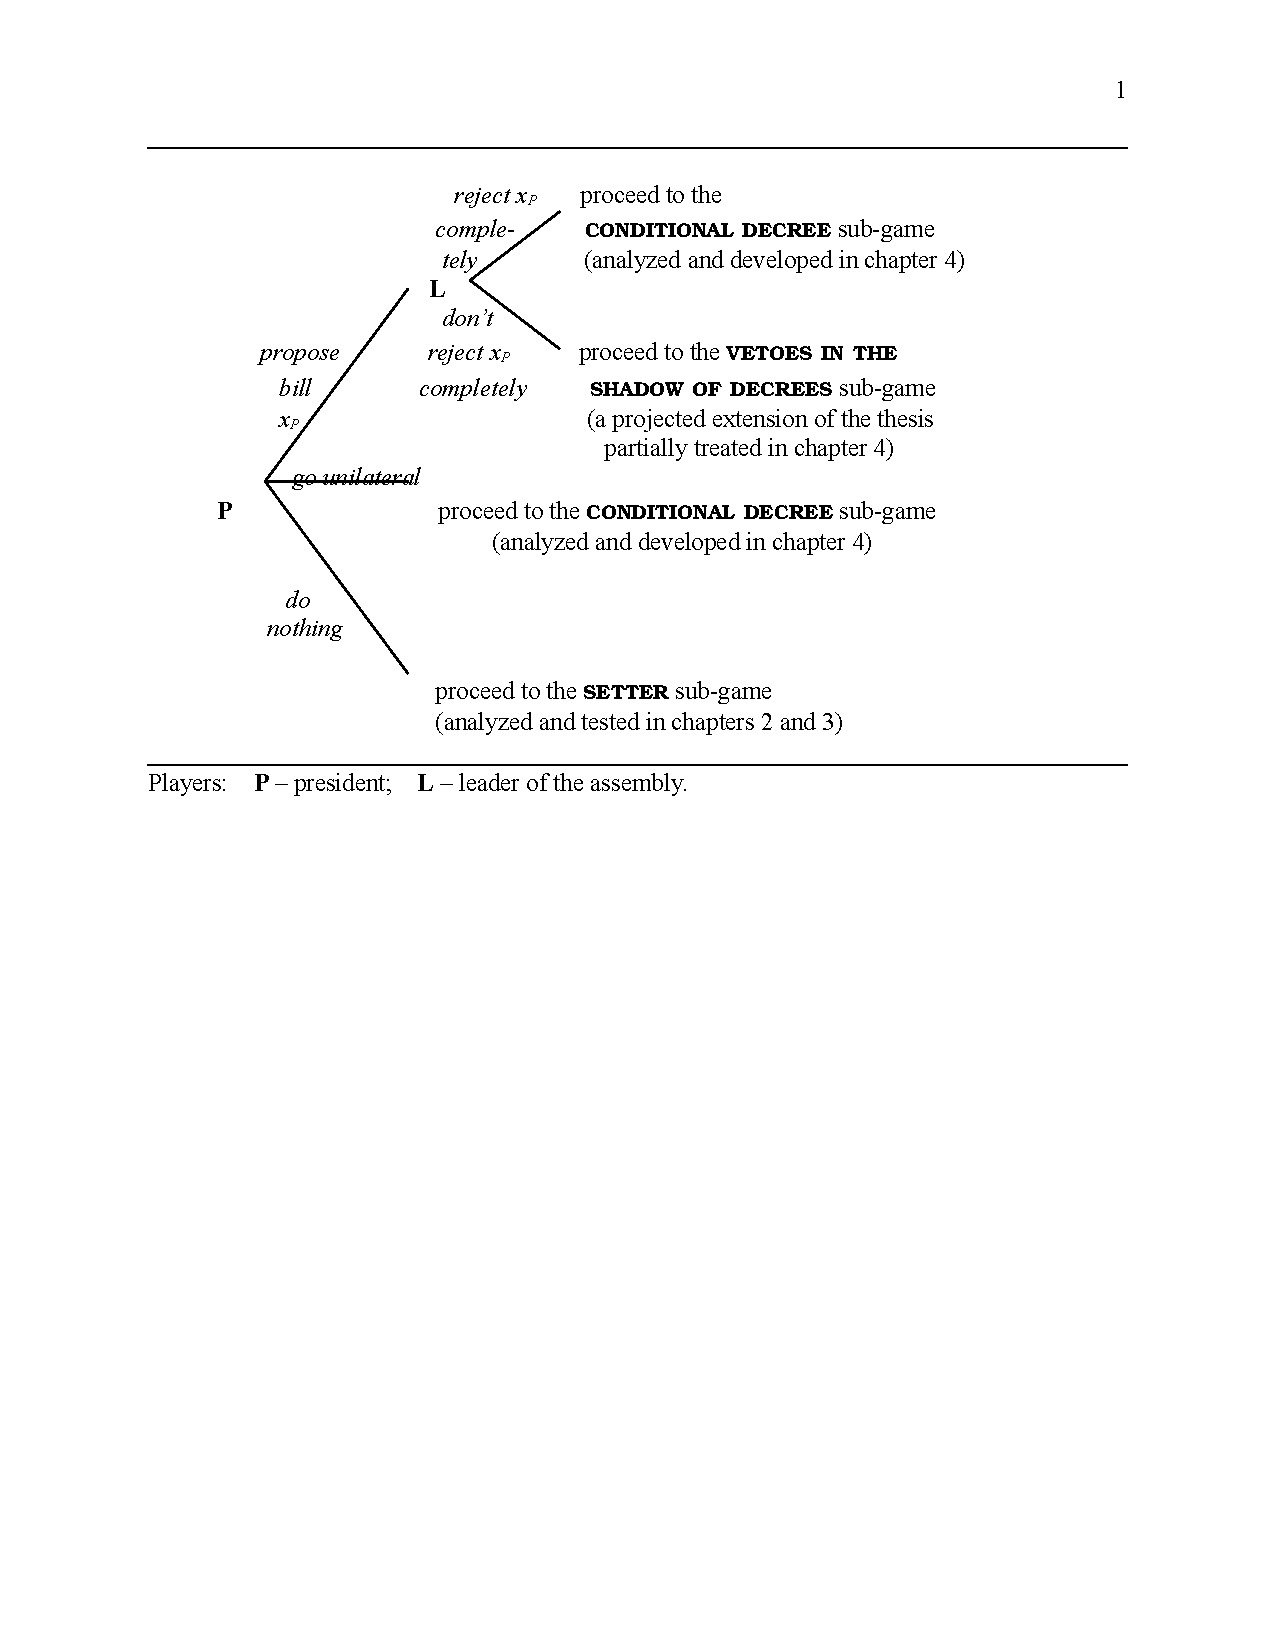
\includegraphics[width=\textwidth]{amplifiedGamePrunedOld.pdf}
 \caption{Amplified SoP and its sub-games}\label{f:amplifiedGamePruned}
 \end{center}
\end{figure}

One theme appeared in the discussion of the sub-games: motivation.  When we see a chess player take the white knight with the black rook it is not hard to infer what motivated black's move.  Black's intention is unlikely to be the knight in question, but to reduce the offensive capacity of the white player while increasing the assault on the white king.  In the legislative process games I sketched above, such inferences are harder to come up with.  Or, more precisely, there are alternative plausible rationalizations of the motivation behind players' moves.  

In particular, what can we infer from observable instances of conflict between the executive and the legislative branches of a sop government?  If we are to take conflict as a symptom of something taking place in the system, what should that something be?  What can be inferred from watching a president veto a bill or an assembly kill an executive initiative?  In my elaboration of the sub-games I discussed three conjectures on motivation: conflict as a symptom of acute polarization (à la Linz); conflict as a bargaining ploy in search of policy payoffs (à la Cameron); and conflict as a publicity stunt in search of electoral payoffs (my contribution to the debate).  

In chapter 7 I will elaborate a discussion on motivation around three major points.  First, motivation provides testable clues about the determinants of inter-branch conflict.  Why do presidents and legislatures struggle?  Second, different interpretations of motivation have different implications for the performance of sop systems.  If polarization is the major cause of inter-branch quarrels, then conflict should be taken with alarm; if, on the other hand, bargaining is the motive, then conflict is a sign that the system is working as intended.  Third, by underlying motivation it becomes possible to bridge a major gap between two literatures that have been treating with the same topic (the legislative process under sop) in near isolation from each other.  Comparative politics and Anglo-American politics literature, when seen through the lens of motivation, are not that stranger to each other.  A unified model of the legislative process under sop is conceivable, very much in the spirit of Strom's \citeyearpar{strom.1990b} unified theory of competitive political parties and of many others \citep{cox.mccubbins.1993,kingdon.1977,schlesinger.1984}.  Cameron's bargaining approach and Linz's polarization approach will become special cases of a more general theory of motivation in the legislative process.  

Last, the unified model will also provide some leverage to connect the literature on the legislative process with another prominent literature in Comparative politics, that on democratic breakdown \citep{linz.stepan.1978,odonnell.1973}.  

\section{A research design}

I will adopt an empirical approach to the legislative process in sop systems.  The guiding idea is the following: To the extent that vetoes and unilateral moves are a mixture of bargaining ploys (in search of policy payoffs) and publicity stunts (in search of electoral payoffs), and not evidence of Linz's irreconcilable differences, then there should be systematic patterns in their use.  The detection of such patterns would be important evidence that Latin-American systems of sop operate ``within the rules''.  

Traditional Latin-American area studies have often argued that the region is a land with a strong man tradition, and this trait is the origin of many political peculiarities.  One such peculiarity, the literature suggested repeatedly, is a propensity for the executive to annul the separation of power provisions written in the constitution \citep{dealy.1992,segovia.1975,meyer.reyna.1989,garcia.hamilton.1990,wiarda.1992}.  ``No appraisal of the democratic and liberal character or operation of a regime of this nature should be based on the effectiveness of congressional checks on the president's broad powers.  Such a criterion, which is valid for the United States, is not for Latin America'' (Lambert \citeyear[][19]{lambert.1971}; see also Tena Ramírez \citeyear{tena.1949}, Jorrín \citeyear{jorrin.1953}; Mecham \citeyear{mecham.1959}; Anderson \citeauthor{anderson.1967}; Carpizo \citeyear{carpizo.1978}; O'Donnell \citeyear{odonnell.1994}).  Stories of executive predominance are abundant in textbooks and research published thirty five years ago---some do not hesitate in depicting Latin-American presidents as ``viceroys'' \citep[][291]{scott.1958}, ``monarchs'' \citep[][410]{edelmann.1969}, or even ``czars'' \citep[][225]{pierson.gil.1957}.  

One way of making sense of the research to follow is by means of the following questions.  Is separation of power a real, functioning, part of Latin-American political systems, or is it just for show?  If this part is real, what effects does it produce?  If the fundamental constitutional provisions serve more than ``a decorative function in a caudillo's palace'' \citep[][399]{lambert.gandolfi.1987} then inter-branch conflict should follow systematic patterns produced by the necessity of bargaining and position-taking between an executive and a legislature that are independent from each other.  Ample evidence of these systematic patterns has been found in other systems of separation of power: the U.S. and its states \citep[see][]{cox.kernell.1991,alt.lowry.1994,poterba.1994,cameron.2000}.  Is Latin-American separation of power fundamentally different from the system that inspired it 180 years ago?  To what extent can we consider Anglo- and Latin-American political systems to be alike?  

My approach to answering these research questions is to explicitly model the separation of power, predict patterns of conflict under different conditions, and test with evidence from relevant empirical referents.  The dependent variable throughout the thesis is the incidence and nature of executive-legislative conflict.  Using the framework that I outlined in this chapter, I pay attention to three classes of explanatory factors of this phenomenon.  Firstly, the formal rules of the legislative process in different systems of separation of power, in particular the rules that govern the rejection of legislative proposals made by the other branch (legislative and executive vetoes) and rules that establish means to overcome such rejections (executive decrees and veto overrides).  Secondly, the alignment of preferences among those who play by these rules, particularly the partisan composition of the branches.  Thirdly the impetus of elected officials towards position-taking, in particular the urgency raised by nearing elections to advocate and loudly voice policy palatable to constituents.  I will be interested in testing the extent to which these three classes of factors shape the occurrence of executive-legislative conflict in systems of sop in the Americas.  Formal rules, the partisan alignment, and the electoral timetable thus become the specific details of strategic game forms allowing me to draw testable predictions.  

The Systematic Effects Hypothesis.  Presidents should veto a bill when that veto might be sustained, or to stake out an electorally advantageous position; otherwise, the assembly gets its way, through threatened or actual override.  Assemblies should veto when they might succeed, or to stake out an electorally advantageous position; otherwise, the president gets his way, through threatened or actual decrees.  Vetoes should vary systematically with unilateral requirements, with the strength in the incentive to advertise a position, with the partisan profile of the branches of government, with each side's uncertainty about the other's preferences, and so forth.  All of these sorts of patterns have been found in the U.S., where democracy is the ‘only game in town' \citep{przeworski.1991} and politicians for the most part abide by its rules.  Does ‘real politics' in Latin-American systems flow around or behind the separation of power, so that the sort of careful and systematic navigating around vetoes that one observes in the U.S. is unnecessary, hence unobserved?  

To the extent that the Linzian perspective on irreconcilable differences is correct, and that separation of power is pure democratic window-dressing, the Systematic Effects Hypothesis should fail miserably.  My research is an attempt to determine this controversy empirically.  

\section{Plan of the book}

Chapter 2 extends Romer and Rosenthal's \citeyearpar{romer.rosenthal.1978} agenda-setter model to players with dual motivation (to bring home policy desired by constituents and to advocate and publicize positions dear to them).  The revised position-taking setter model supports a positive incidence of vetoes in equilibrium.  Chapter 3 places deductive predictions from the revised model against the empirical record.  Data on executive veto incidence in U.S. state governments serves to put the revised model to a thorough test, which it passes quite successfully.  Chapter 4 follows Argentina's legislative process longitudinally.  The chapter synthesizes dispersed evidence on executive decrees, on failed executive bills, and on successful bills.  The result is a dataset with which veto incidence can be estimated for both the executive and Congress.  Chapter 5 analyzes a case of real bargaining between the president and Congress in Argentina over pensions reform.  The congressional veto can be used to extract concessions from the executive, the narrative suggests; a mirror image of Cameron's story for the U.S.  Chapter 6 offers two case histories of vetoes as publicity stunts intended to gain votes at the next election, developing the contrast between the three perspectives on motivation (Cameron, Linz, Magar).  Chapter 7 concludes by returning to the big picture.  The chapter sketches the bases for a unified model of the legislative process.  


% Extra stuff…
% 	The equilibria of the games.  If the games were, each, repeated infinitely by players whose only motivation is to win the game, would there be some predictable patterns?  What can be said about the topic of this work: the incidence of vetoes?  Answering these questions requires, in the parlance of game theory, to find the set of players' best reply strategies to those of the opponents---otherwise known as equilibria---of each model.  The specification of equilibrium strategies necessitates additional assumptions such as (a) what does it mean to "win” the game (i.e. what are players' goals); (b) how much do players' know/see about each other at each step of the game (i.e. what are the informational premises of the interaction); and others of a more technical nature.  This set of additional assumptions interacts with the rules set-forth so far to guide players into different strategic behavior, and different premises lead to different solutions of the game.  

% no sé donde poner esto; probablemente en un capitulo de Linz vs Cameron	Some have urged a constitutional reform in the U.S. to make government more effective [e.g. \Sundquist, 1986 #142]; counter-arguments reminded us that immobilism is the result of the choice checks and balances by the constitutional-writers to safeguard the rights of citizens [e.g. \Cox, 1991 #140].  The response to Linz's critique of presidential democracy follows basically the same train of thought: separation of power involves tradeoffs.  

% 	The equilibrium of the sub-game is more complex than the previous story suggests, since policy xP is endogenous in the model and thus needs to be described as part of an equilibrium strategy.  A full analysis of the vetoes in the shadow of decrees sub-game will be the topic of chapter 4.  

% tmp par	The weighted average approach to motivation, despite its tentativeness, allows to adopt an empirical approach to the legislative process in SoP systems.  Although little is said about the value of α and its determinants, to the extent that vetoes and unilateral moves are a mixture of bargaining ploys (in search of policy payoffs) and publicity stunts (in search of electoral payoffs), and not evidence of Linz's irreconcilable differences, then there should be systematic patterns in their use.  The details of “deadlock” are in whether the different safety valves of SoP systems can operate or not; if they can, in whether they are used or not.  The detection of such patterns is important as evidence that Latin-American government operates “within the rules”, that separation of power is a real, functioning part of Latin-American systems---and not mere democratic window-dressing, as many have to claimed.  



%%% Local Variables: 
%%% mode: latex
%%% TeX-master: "master"
%%% End: 
